\documentclass{article}
\usepackage[margin=.5in]{geometry}
\usepackage{graphicx, dblfloatfix}
\usepackage{amsmath, amssymb, amsfonts, mathrsfs, mathtools, physics}
\usepackage{gensymb}
\usepackage[english]{babel}
\usepackage[autostyle, english = american]{csquotes}
\usepackage[normalem]{ulem}
\usepackage[title,titletoc,toc]{appendix}
\usepackage{pgfplotstable}
\usepackage{array, booktabs, colortbl, caption}
\usepackage{braket}
\MakeOuterQuote{"}

\newcommand{\redchi}{$\tilde{\chi}^2\,$}
\renewcommand{\vec}[1]{\mathbf{#1}}

\title{Specific Heat of Metals}
\author{Alejandro Legarda}

\begin{document}
\raggedright
\maketitle

\begin{abstract}
We investigate the molar specific heat capacity, $c_m$, of Nickel and Niobium from a range of about 5 degrees Kelvin to room temperature. The plots show a rapid rise in $c_m$ until they plateau at about $T > 200k$. We observe a discontinuity in the $c_m$ of Niobium at the superconducting temperature $T_c = 8.75 \pm 0.5$. We determine Debye temperatures for the two samples using a linear fit of low (but not superconducting) temperature $c_m$s. These values fall within $1\sigma$ of the literature, but our fits yield anomalous y-intercepts, particularly for Niobium. We obtain the ratio $\frac{c_{se}}{c_{ne}} = 6 \pm 2$ which is inconsistent with theory but is within the right order of magnitude.
\end{abstract}
	
	
\tableofcontents
\newpage

\section{Theory}

\subsection{Specific Heat Capacity}

The specific heat capacity, $c$, of a material, is a measure of the amount of energy per degree kelvin needed to change the temperature of the material. The more general hear capacity is given by

\begin{equation}
	C = \frac{\partial E}{\partial T}.
\end{equation}

For a specific material, the specific, molar, heat capacity is given by

\begin{equation}
	c_m = \frac{C}{N},
\end{equation}

where N is the number of moles.

\hspace{.25cm}

In solids, thermal energy is stored in primarily two ways, or as two distinct capacities: first, as the excitation of lattice vibrations (phonons), which we will designate by $c_p$, and as (present only in metals) energy held by the conduction electrons which we will designate by $c_e$. Let us consider the contribution due to lattice vibrations first.
According to the Debye model, the number of vibrational modes in a lattice increases as the square of the vibrational frequency, $\omega$, up to a maximum value, the Debye frequency, $\omega_D$. (See Fig. 1.) Therefore, at low temperatures, only some of the modes are available (those with energies $E \leq k_B T$), and adding heat to the system goes into exciting new vibrational modes. This low temperature lattice vibration contribution to the molar heat capacity goes as

\begin{equation}
	c_p = \frac{12 \pi^4 N_A k_B}{5}(\frac{T}{\Theta_D})^3,
\end{equation}

where $N_A$ is Avogadro's number, $k_B$ is the Boltzmann constant, and $\Theta_D$ is the Debye temperature.

\begin{figure}[!htb]
	\centering
	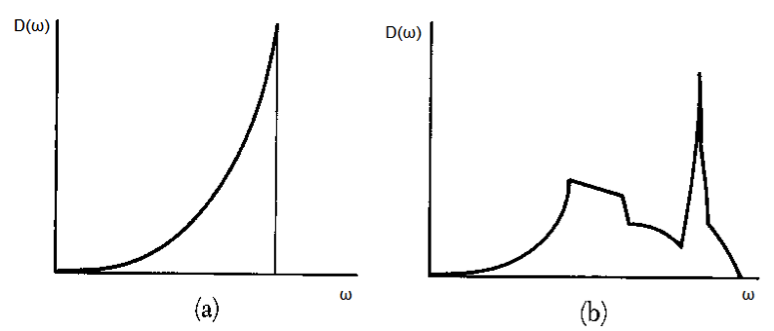
\includegraphics[scale=1.]{plots/fig_1.png}
 	\label{debye}
	\caption{(a) Debye model density of states. (b) A realistic density of states.\cite{lab manual}}
\end{figure}

Above the Debye temperature, all modes are available and therefore adding heat to the system only increases the amplitude of already excited modes. In this regime, there is no temperature dependence at all and the lattice vibration contribution to the specific heat is predicted to approach the constant value

\begin{equation}
	c_p = 3 N_A k_B \approx \frac{25 J}{mol K},  (T > \Theta_D).
\end{equation}

In metals, we also consider the contribution due to energy held in the conduction electrons, which is proportional to temperature. Most electrons in a metal are localized near the atoms in the valence band, but the electrons on the conduction band may absorb or emit photons of energy $k_B T$. This contributions is linearly proportional to temperature, $c_e = \gamma T$. We then have the total specific heat as a function of T,

\begin{equation}
	c(T) = c_p(T) + c_e(T) = \frac{12 \pi^4 N_A k_B}{5}(\frac{T}{\Theta_D})^3 + \gamma T = \alpha T^3 + \gamma T, (T > \Theta_D).
\end{equation}

The two terms can be separated by plotting $\frac{c}{T}$ against $T^2$ at low temperatures (below $T \approx 18 K$ for our experiment), but above $T_C$, the superconducting transition temperature. The $T = 0$ intercept of this plot yields $\gamma$, while the slope yields $\alpha$ (and therefore the Debye temperature)\cite{lab manual}.


\subsection{Heat Capacity in the Superconducting State}

Niobium becomes superconducting at $T_C \approx 9 K$. At this critical temperature, an energy gap opens up in the electron band structure as a result of Cooper pair formation, and there is a sudden change in the way electrons carry energy. This leads to a discontinuity in the specific heat such that the specific heat jumps up in value at $T_C$, but then falls to zero more quickly with decreasing temperature than a normal conductor. (See Fig. 2.) This change, however, affects only the electronic contribution, $c_e$; the lattice vibration contribution to the specific heat, Eq .(4), remains unchanged through the transition. \cite{lab manual}

\begin{figure}[!htb]
	\centering
	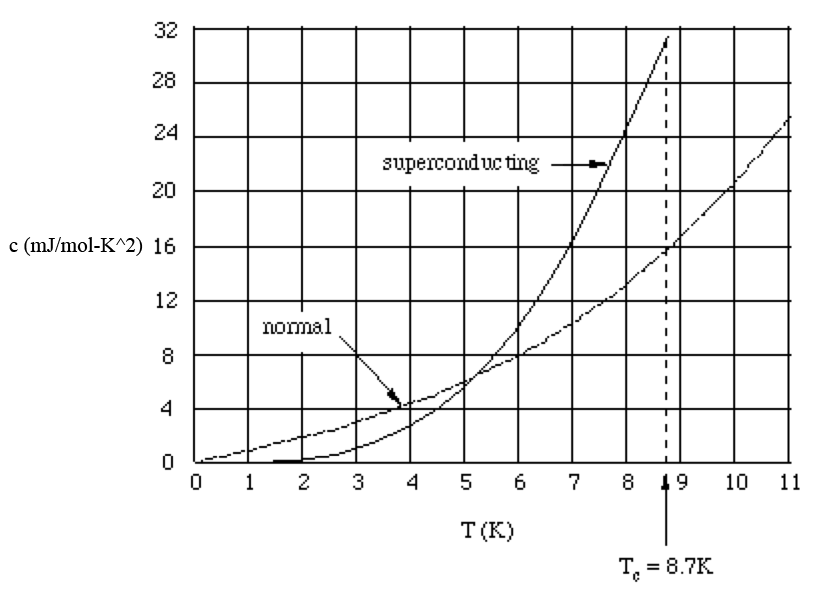
\includegraphics[scale=.5]{plots/fig_2.png}
 	\label{super}
	\caption{Specific heat of normal and superconducting niobium at low temperatures. \cite{lab manual}}
\end{figure}

The Bardeen-Cooper-Schrieffer (BCS) theory of superconductivity predicts that the electronic contribution to the superconducting specific heat is

\begin{equation}
	c_e =  c_0 e^{-\frac{2 \Delta}{T}},
\end{equation}

where $\Delta$ is the superconducting band gap energy. This band gap is nearly constant at low temperatures, but diverges as $T \rightarrow T_C$. We can investigate the ratio of the superconducting to normal specific heats right at the transition between the two states. In the normal state, the electron contribution is $c_{ne} = \gamma T_C$, whereas in the superconducting state, the electron contribution is the measured value, $c_s$, minus the known lattice vibration contribution, $\alpha T_C^3$, such that $c_{se} = c(T = T_C) - \alpha T_C^3$. The BCS predicted ratio of these two quantities (which is expected to be the same for all superconductors) is

\begin{equation}
	\frac{c_{se}}{c_{ne}} =  2.43.
\end{equation}


\section{Experimental Method}
\subsection{Apparatus}

Two cylindrical samples of Ni and Nb, about 1" long and 0.5" diameter, are mounted in a stainless steel tube as shown in Fig. 3. Their masses are $27.89 \pm 0.05 g$ for Ni and $24.20 \pm 0.05 g$ for Nb. The samples are thermally insulated as best as can be managed in an undergraduate laboratory setting - there will be some thermal transfer, and therefore uncertainty due to the wiring of the apparatus. The wiring is responsible for delivering a pulse of known voltage to the source. Current across the source is measured, as is the change in temperature due to the pulse. From current, resistance of the wire (which varies with temperature) and voltage we can calculate the energy delivered to the sample, and knowing the change in temperature, we are able to calculate the specific heat capacity of the sample. The change in temperature is read off a silicone diode. We cool the samples by pouring liquid nitrogen into the outer glass tube of the apparatus. This gets us to about 100 degrees Kelvin. We use liquid helium, delivered into the inner glass tube (which surrounds the steel tube), to cool the samples down to about 5 degrees.

\begin{figure}[!htb]
	\centering
	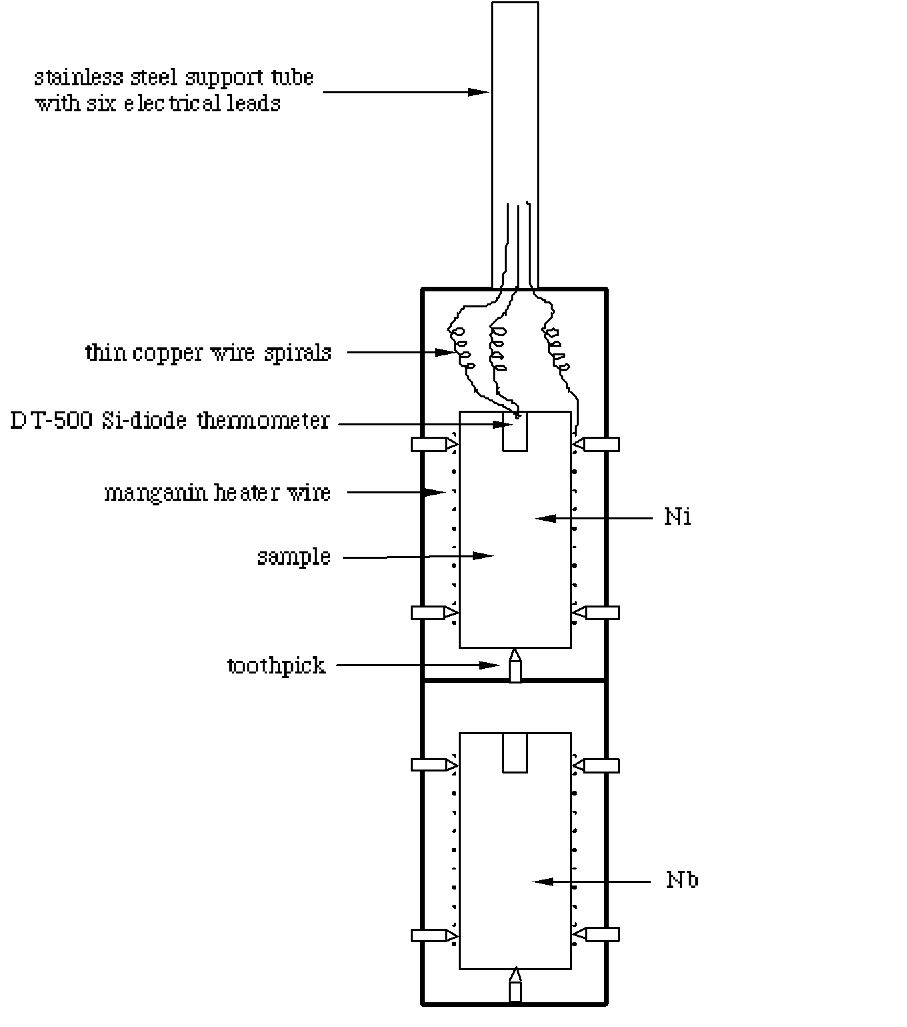
\includegraphics[scale=.75]{plots/apparatus.png}
 	\label{apparatus}
	\caption{Niobium and nickel samples are mounted above one another on wooden toothpicks. \cite{lab manual}}
\end{figure}

\subsection{Cooling}

As mentioned, a wide range of temperatures can be covered by simply pouring liquid nitrogen into the outer dewar of the apparatus. However, liquid helium is necessary to reach the lower temperatures. The method for safely adding liquid helium is as follows. First, the system is flushed with helium so that its atmosphere, and that of the tubing is almost solely helium atoms. A hook-like tube with a coiled mid-section is fed into the vacuum jacket of the inner dewar of the apparatus and into the liquid helium container. This inner vacuum jacket must first be pumped with a forepump, backfilled with air and then pumped again at least three times. This ensures that thermal isolation is as good as we can get it. Residual air will freeze when the liquid helium is introduced, providing a strong vacuum in the jacket. The turbo-pump valve is opened to allow thermal transfer between the sources and the liquid helium/nitrogen.


\section{Data}


We use recordings of temperature and voltage, knowing the resistance of the leads that go to the sample, to calculate the energy deposited in the sample. Using the change of temperature, we calculate the heat capacity, C, of the sample.

\begin{equation}
	C = \frac{I*V - I*R}{\Delta T},
\end{equation}

where R is the resistance of the leads, which can vary with temperature. We calculate uncertainties using the Taylor propagation method, \cite{taylor}

\begin{equation}
	\delta C = \sqrt{(\frac{IV - I^2R}{{\Delta T}^2})^2 (\delta \Delta T)^2 + (\frac{I - I^2R}{\Delta T})^2 (\delta V)^2 + (\frac{V - 2IR}{\Delta T})^2 (\delta I)^2}.
\end{equation}

Table one shows some sample data at liquid nitrogen ranges.

\begin{table}[]
\centering
\caption{Sample Data}
\label{sample}
\begin{tabular}{@{}llllll@{}}
\toprule
Metal & Initial T & $I (mA) \pm 0.000001$ & $V \pm 0.01$ & $\Delta T$    & $C$                   \\ \midrule
Nb    & 294.3     & 0.199054              & 17.47        & $2.4 \pm 0.1$ & $0.00145 \pm 0.0006$  \\
Nb    & 112.6     & 0.199105              & 17.35        & $4.1 \pm 0.1$ & $0.00842 \pm 0.00002$ \\
Ni    & 294.3     & 0.199051              & 17.09        & $1.3 \pm 0.1$ & $0.0026 \pm 0.0002$   \\
Ni    & 109.1     & 0.199091              & 16.49        & $2.5 \pm 0.1$ & $0.00131 \pm 0.00005$ \\ \bottomrule
\end{tabular}
\end{table}

At low temperatures, DAQ software is used. In the range of 4-20 K, we rely on the software to provide a best fit to the linear rise in temperature due to the pulse. There is a 5 second pre-pulse and a 5 second post-pulse around the 5 seconds of actual energy delivery. The gradient of the fit between the pre and post pulses is a measure of the heat capacity. We take a random (Nickel) data point in order to test the software's gradient calculation. We apply our own piecewise linear fit using python.


\begin{table}[]
\centering
\caption{Software and Manual Slope Calculations}
\label{low-table}
\begin{tabular}{@{}llll@{}}
\toprule
           & Pre-Pulse           & Heat Pulse          & Post-Pulse          \\ \midrule
Software   & $0.0065 \pm 0.0005$ & $0.0098 \pm 0.0006$ & $0.0060 \pm 0.0004$ \\
Manual Fit & $0.006 \pm 0.001$   & $0.010 \pm 0.001$   & $0.006 \pm 0.001$   \\ \bottomrule
\end{tabular}
\end{table}

\hspace{.25cm}

Comparing the data in Table 2 and looking at Figure 4, we can be confident that the software produces adequate linear fits, since our values and the software's values are well within $1\sigma$ from each other.

\hspace{.25cm}

In order to calculate molar specific heat capacity, we must first calculate the number of moles per sample. The masses with uncertainties were given above, and they yield $N_{Ni} = 0.4751 \pm 0.0009 mol$ for Nickel and $N_{Nb} = 0.2605 \pm 0.0005 mol$ for Niobium. We can then plot molar specific heat capacity against temperature for both samples.

\begin{figure}[!htb]
	\centering
	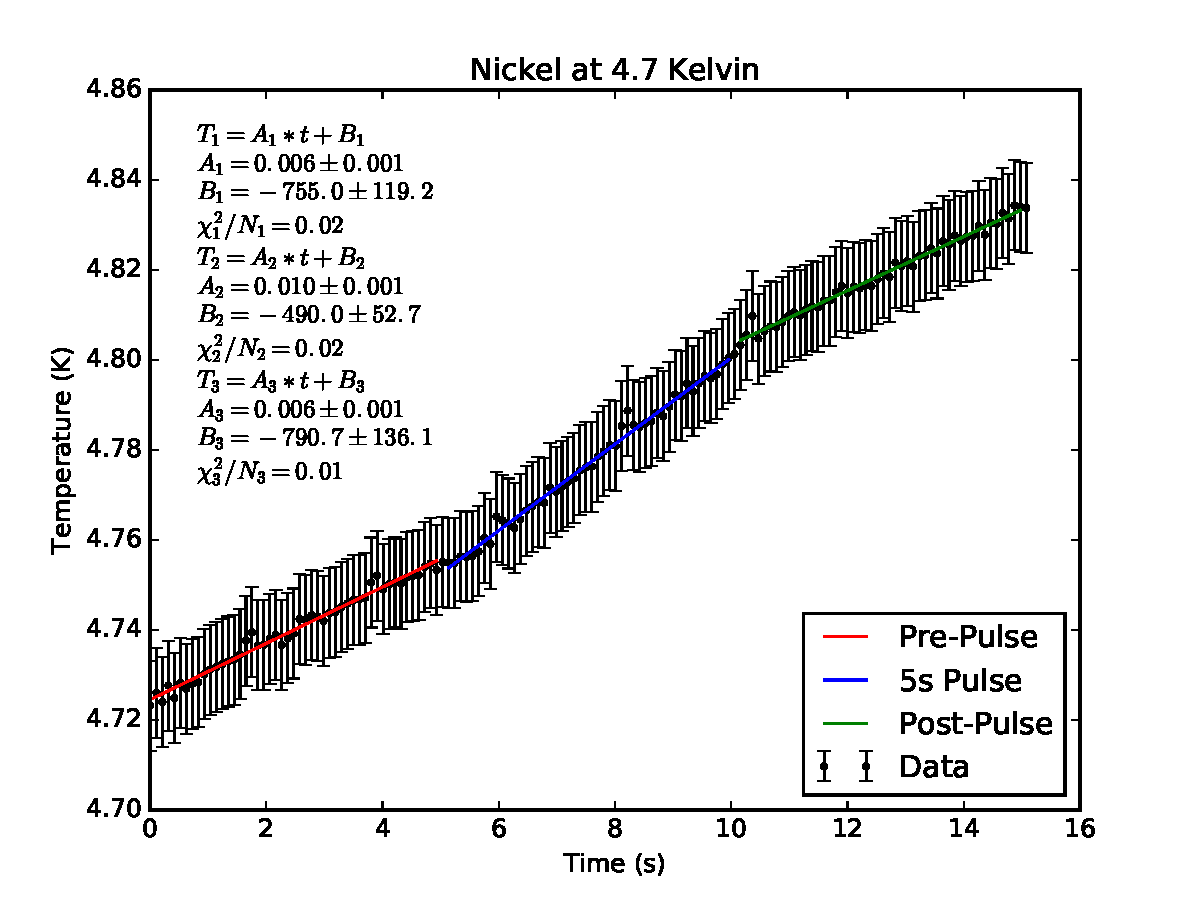
\includegraphics[scale=.75]{plots/low-fit.pdf}
 	\label{lNickel}
	\caption{A piecewise linear fit to the temperature data form a random pulse. The error bars seem to large, but come directly from the software. This helps illustrate the fact that uncertainty in temperature measurements is the largest source of systematic error.}
\end{figure}

\begin{figure}[!htb]
	\centering
	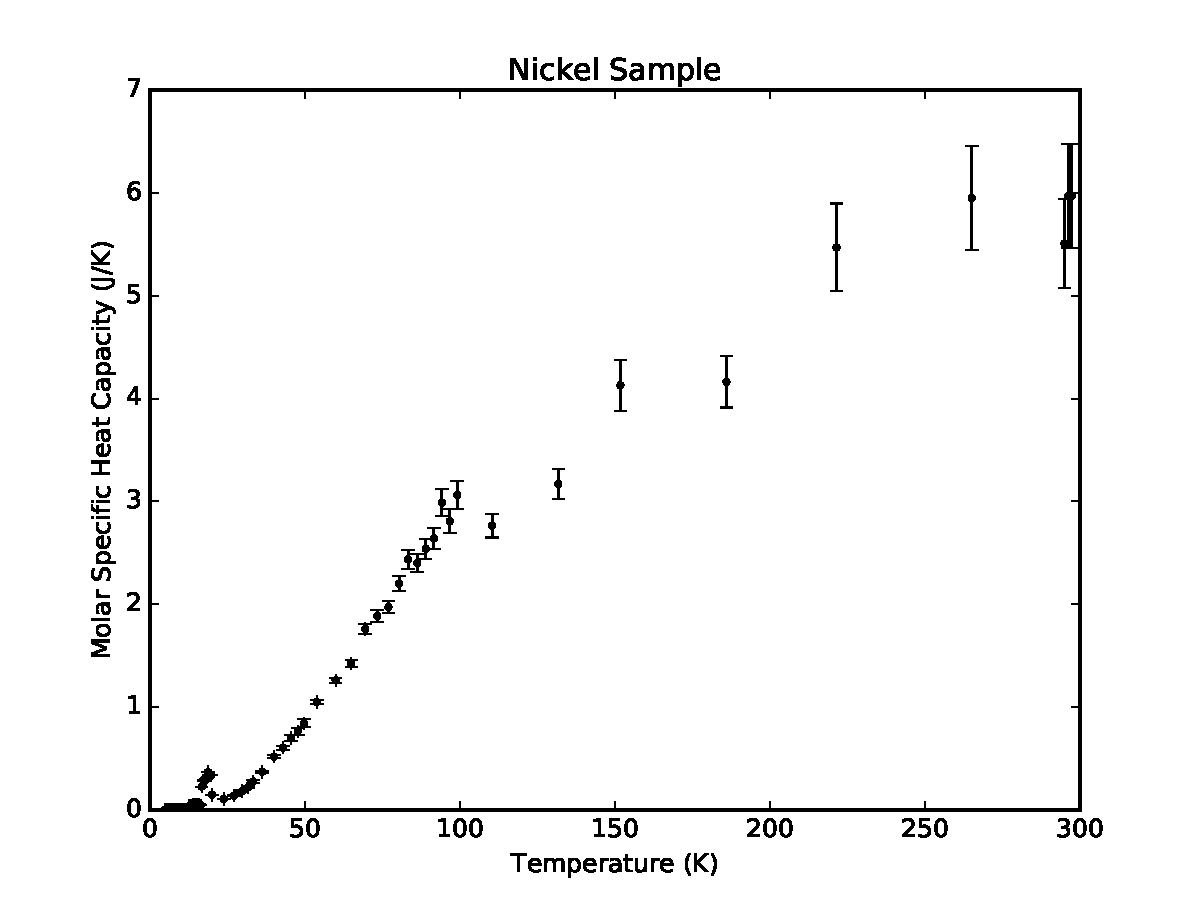
\includegraphics[scale=.75]{plots/Ni.pdf}
 	\label{Ni}
	\caption{Molar specific heat capacity for Nickel.}
\end{figure}

\begin{figure}[!htb]
	\centering
	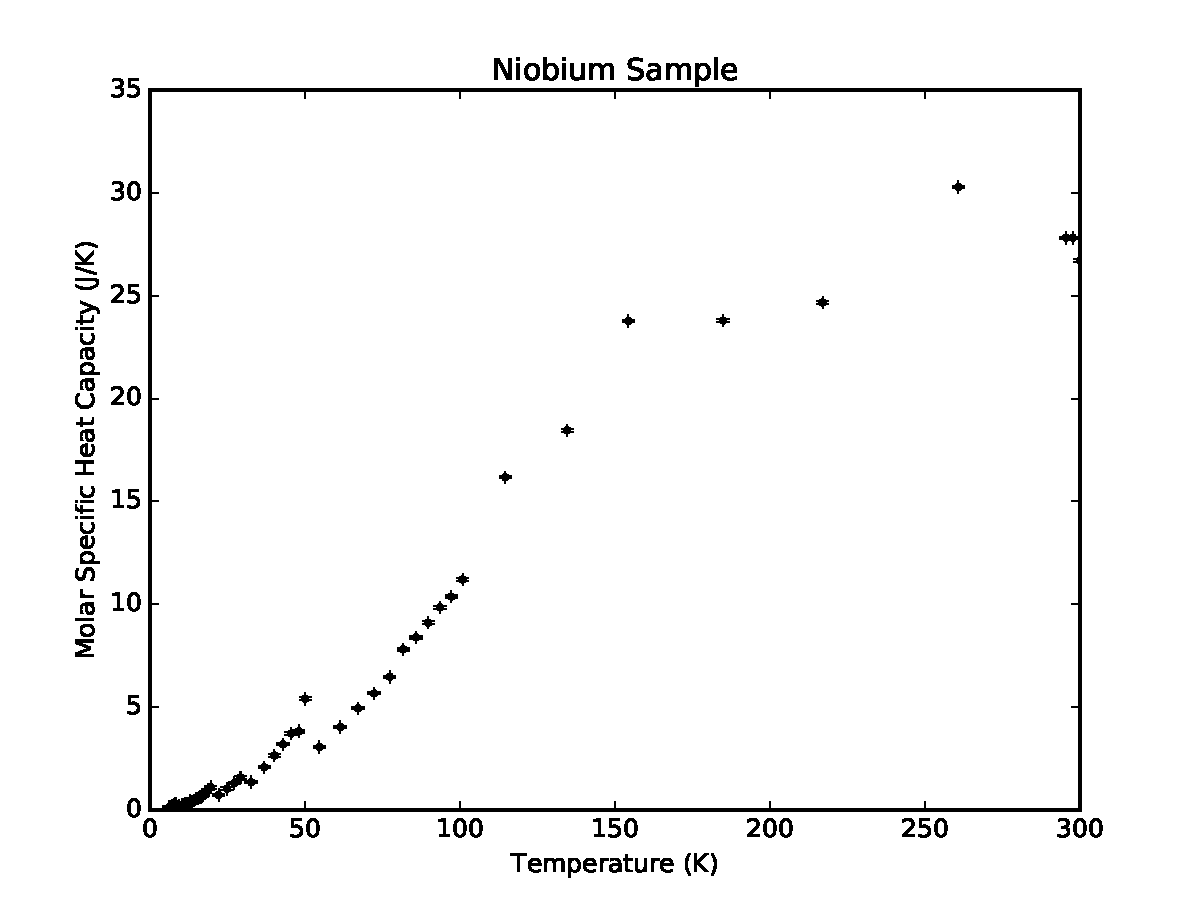
\includegraphics[scale=.75]{plots/Nb.pdf}
 	\label{Nb}
	\caption{Molar specific heat capacity for Niobium. A discontinuity is seen at $T = T_c = 8.75 \pm 0.5$K, indicating a phase transition (from supersolid to solid). This values falls just within $1\sigma$ of the literature value of $T_c = 9.25$K. $T_c$ was determined by looking at the data table, and therefore the uncertainty is about the difference in temperature between $T_c$ and adjacent data points. The plateau is consistent with the prediction of equation (4) for high temperatures.}
\end{figure}

One can interpret from these plots that both Nickel and Niobium specific heat capacities begin to plateau around 200 degrees Kelvin. We can select the superconducting portion of the Niobium data and do a linear fit of the form of equation (5). This will allow us to extract slope and intercept parameters, with which we can determine $\Theta_D$.

\begin{figure}[!htb]
	\centering
	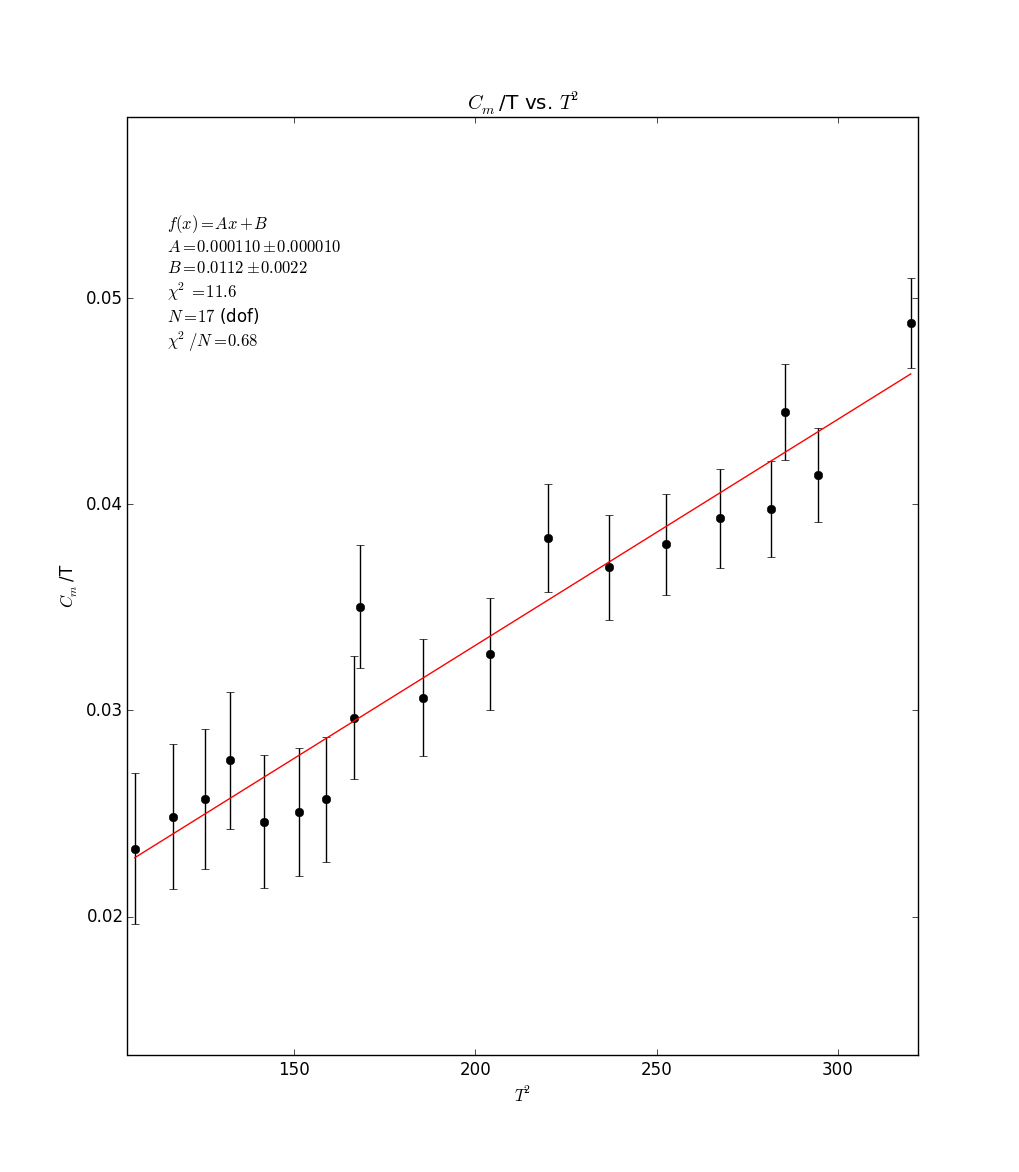
\includegraphics[scale=.5]{plots/linfit.png}
 	\label{Nb}
	\caption{Linear fit for cold but not superconducting region of Niobium. We obtain $\alpha = 0.00011 \pm 0.00001JK^{-1}; \gamma = 0.0112 \pm 0.002$J. Since we are not ever past the Debye temperature, $c_m$ does not fully plateau on this plot.}
\end{figure}

\begin{figure}[!htb]
	\centering
	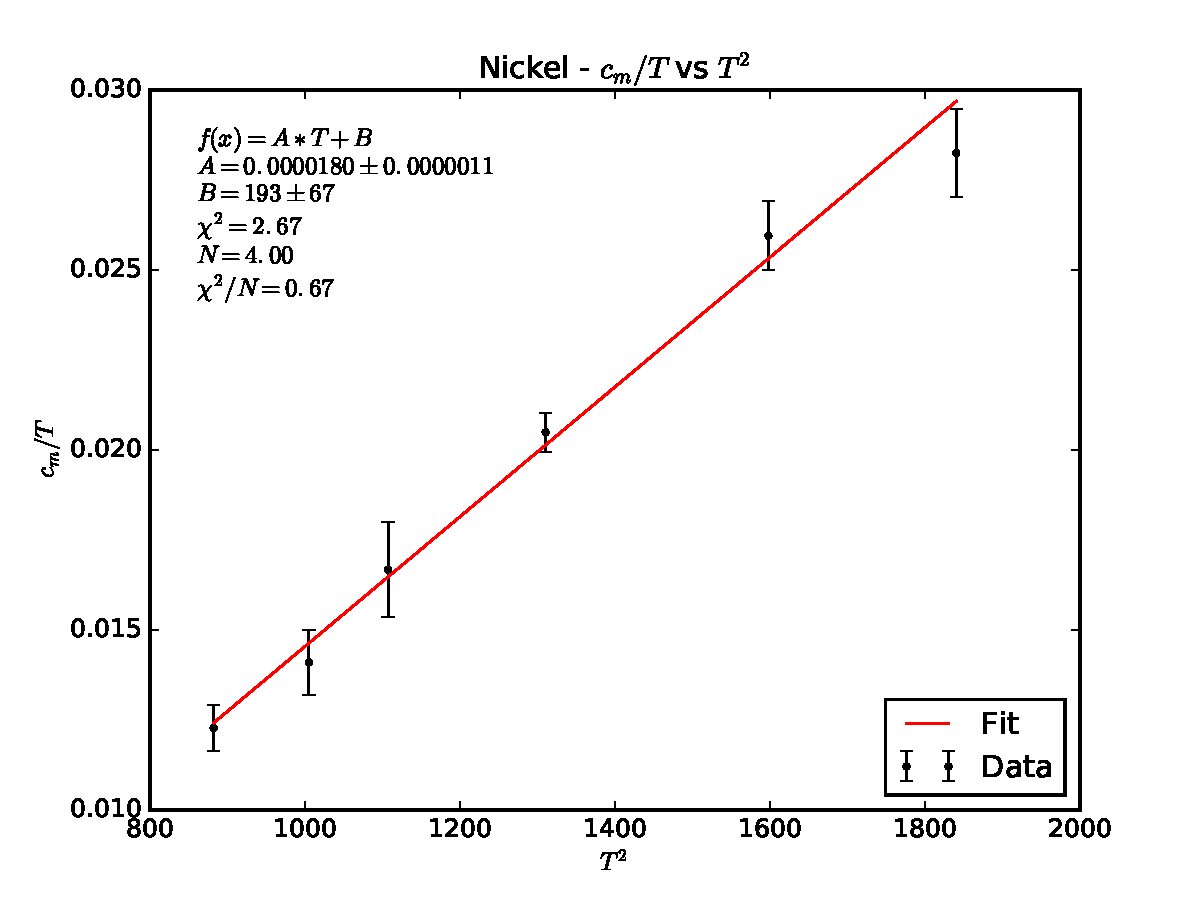
\includegraphics[scale=.75]{plots/Ni_linfit.pdf}
 	\label{Nb}
	\caption{Linear fit for cold but not superconducting region of Nickel. We obtain $\alpha = 0.000018 \pm 0.000001JK^{-1}; \gamma = 190 \pm 70$J. The huge error on our intercept is partly due to the small number of points we have that fit well in this region.}
\end{figure}

We can find $\Theta_D$ by solving the equation

\begin{equation}
	\alpha = \frac{12\pi^4 N_A k_B}{5(\Theta_D)^3}.
\end{equation}

We thus obtain, for Niobium (Fig. 7), $\Theta_D = 260 \pm 20$K. This is within $1\sigma$ of the literature value of $\Theta_D = 275$K. For Nickel (Fig. 8), we obtain $\Theta_D = 480 \pm 30$K. This is within $1\sigma$ of the literature value of $\Theta_D = 450$K. Here, the uncertainties in the slope and intercepts were propagated using standard Taylor methods. Our values of $\gamma$ are $\gamma_{Nb} = 0.11 \pm 0.01$ mJ and $\gamma_{Ni} =11 \pm 2$. Our value for Nickel is within $2\sigma$ of the literature value $\gamma_{Ni} = 7.02$. The value for Niobium is orders of magnitude off, and this suggest some systematic shift in the data, since the $\alpha$ value is reasonable.
\hspace{.25cm}

We can compute $c_{ne}$ and $c_{se}$ from our fit parameters, where

\begin{gather}
	c_{ne} = \gamma T_c \\
	c_{se} = c_s - \alpha T_c^3.
\end{gather}

Where $c_s = c(T = T_c) = 0.23 \pm 0.02 J mol^{-1}$ is the molar specific heat capacity at the superconducting temperature. We thus obtain $c_{ne} = 0.0253 \pm 0.004$ and $c_{se} = 0.16 \pm 0.03$, where 

\begin{equation}
	\delta c_{se} = \delta c_s + \sqrt{(T_c^3)^2*(\delta \alpha)^2 + (2\alpha*(T_c^2))^2*(\delta T_c)}.
\end {equation}

We then obtain $\frac{c_{se}}{c_{ne}} = 6 \pm 2$. This is within $2\sigma$ of the literature value of $\frac{c_{se}}{c_{ne}}=2.8-3.0$. This result reinforces the idea that there is some systematic error somewhere, but that our data shows the relationships well.

\section{Conclusion}

Molar specific heat capacity is at its lowest for the low superconducting temperatures. For Nickel, a drop is then seen before a fairly linear rise, up to the high-T plateau where $c_m$ follows a plateauing square-root functional form. For Niobium, the initial rise is less sharp, and there are one or two state transitions at the low temperatures that cause a discontinuity. At higher temperatures $c_m$ for Nb also plateaus - both do so around 200 degrees Kelvin, although the variance of our data at high temperatures makes it difficult to determine.

\hspace{.25cm}

Our fits are constrained by two things: the number of data points we have and the uncertainty on those points. As already mentioned, we could have used more points in the linear fit region to obtain better fits. Uncertainties were relatively large for temperature measurements, leading to small reduced chi squared values. This source of uncertainty is systematic, and the apparatus could be tested with known temperatures for better calibration. We did note some odd behavior during data-taking: the temperature readings sometimes had systematic jumps well above what the correct values should be. However, these erroneous points were never more than a few of the data points of each run (less than one tenth). Our $\gamma$ values for our fits came out completely wrong. This means that, since our values for $\alpha$ were reasonable, our plots show the correct relationship but are shifted in y by some systematic quantity.


\section{Plots}
\clearpage

\clearpage
\begin{thebibliography}{10}

	\bibitem{lab manual}
		University of Chicago Department of Physics. "Specific Heat of Metals"\\
		https://wiki.uchicago.edu/display/P211manuals/Specific+Heat+Of+Metals. (Accessed May, 2016)

	\bibitem{taylor}
		Taylor, John. \emph{An Introduction to Error Analysis}. Sausalito: University Science Books, 1997.
		
\end{thebibliography}

\end{document}